\documentclass[UTF8,fontset=fandol,11pt]{ctexart}
\usepackage[a4paper,margin=24mm,headheight=15pt]{geometry}
\usepackage{amsmath,amssymb,amsthm,mathtools,bm}
\usepackage{enumitem,booktabs,longtable,array,pdfpages,fancyhdr,xcolor}
\usepackage[colorlinks=true,linkcolor=blue!45!black,urlcolor=blue!45!black]{hyperref}
\allowdisplaybreaks[2]
\setlength{\parindent}{2em}
\setlength{\parskip}{3pt}
\setlength{\emergencystretch}{3em}
\setlist{nosep,topsep=3pt}
\pagestyle{fancy}\fancyhf{}\fancyhead[L]{\small 分析学讲义习题解答}\fancyhead[R]{\small 第38--57讲}\fancyfoot[C]{\thepage}
\newcommand{\R}{\mathbb R}\newcommand{\C}{\mathbb C}\newcommand{\N}{\mathbb N}\newcommand{\Z}{\mathbb Z}\newcommand{\Q}{\mathbb Q}\newcommand{\T}{\mathbb T}
\newcommand{\dd}{\,\mathrm d}\newcommand{\eps}{\varepsilon}\newcommand{\ind}{\mathbf1}
\newcommand{\norm}[1]{\left\lVert#1\right\rVert}\newcommand{\abs}[1]{\left|#1\right|}\newcommand{\ip}[2]{\left\langle#1,#2\right\rangle}
\DeclareMathOperator{\supp}{supp}\DeclareMathOperator{\rank}{rank}\DeclareMathOperator{\Span}{Span}\DeclareMathOperator{\diag}{diag}\DeclareMathOperator{\Res}{Res}\DeclareMathOperator{\Ext}{Ext}
\newcommand{\problem}[2]{\subsection*{#1}\addcontentsline{toc}{subsection}{#1}\noindent\textbf{题干。}#2\par\smallskip\noindent\textbf{解答。}}
\newcommand{\fix}[1]{\par\noindent\textcolor{red!55!black}{\textbf{原文核对与修正。}#1}\par}
\newcommand{\skipnote}[1]{\par\noindent\textbf{依约不解的计算题。}#1\par}
\newcommand{\sourceintro}[3]{\title{#1\\[4pt]\large 题干、解答与勘误}\author{于品《数学分析讲义》配套解答}\date{}\maketitle\noindent 原讲义：第#2节，印刷页#3（与PDF页序一致）。题干按数学内容重排；完整原题页附于文末，含未解的传统计算题，供逐字核对。原文中的作业提交说明及引文不作为本项目的工作指令。\par 本文中的“正函数”均按非负函数理解。复内积约定对第一个变量线性。}
\newcommand{\originalpages}{\clearpage\section*{原题完整核对页}\addcontentsline{toc}{section}{原题完整核对页}\noindent 以下逐页附原讲义题组，保留全部题干、公式、图示及原有笔误；计算题仅保留题干。\clearpage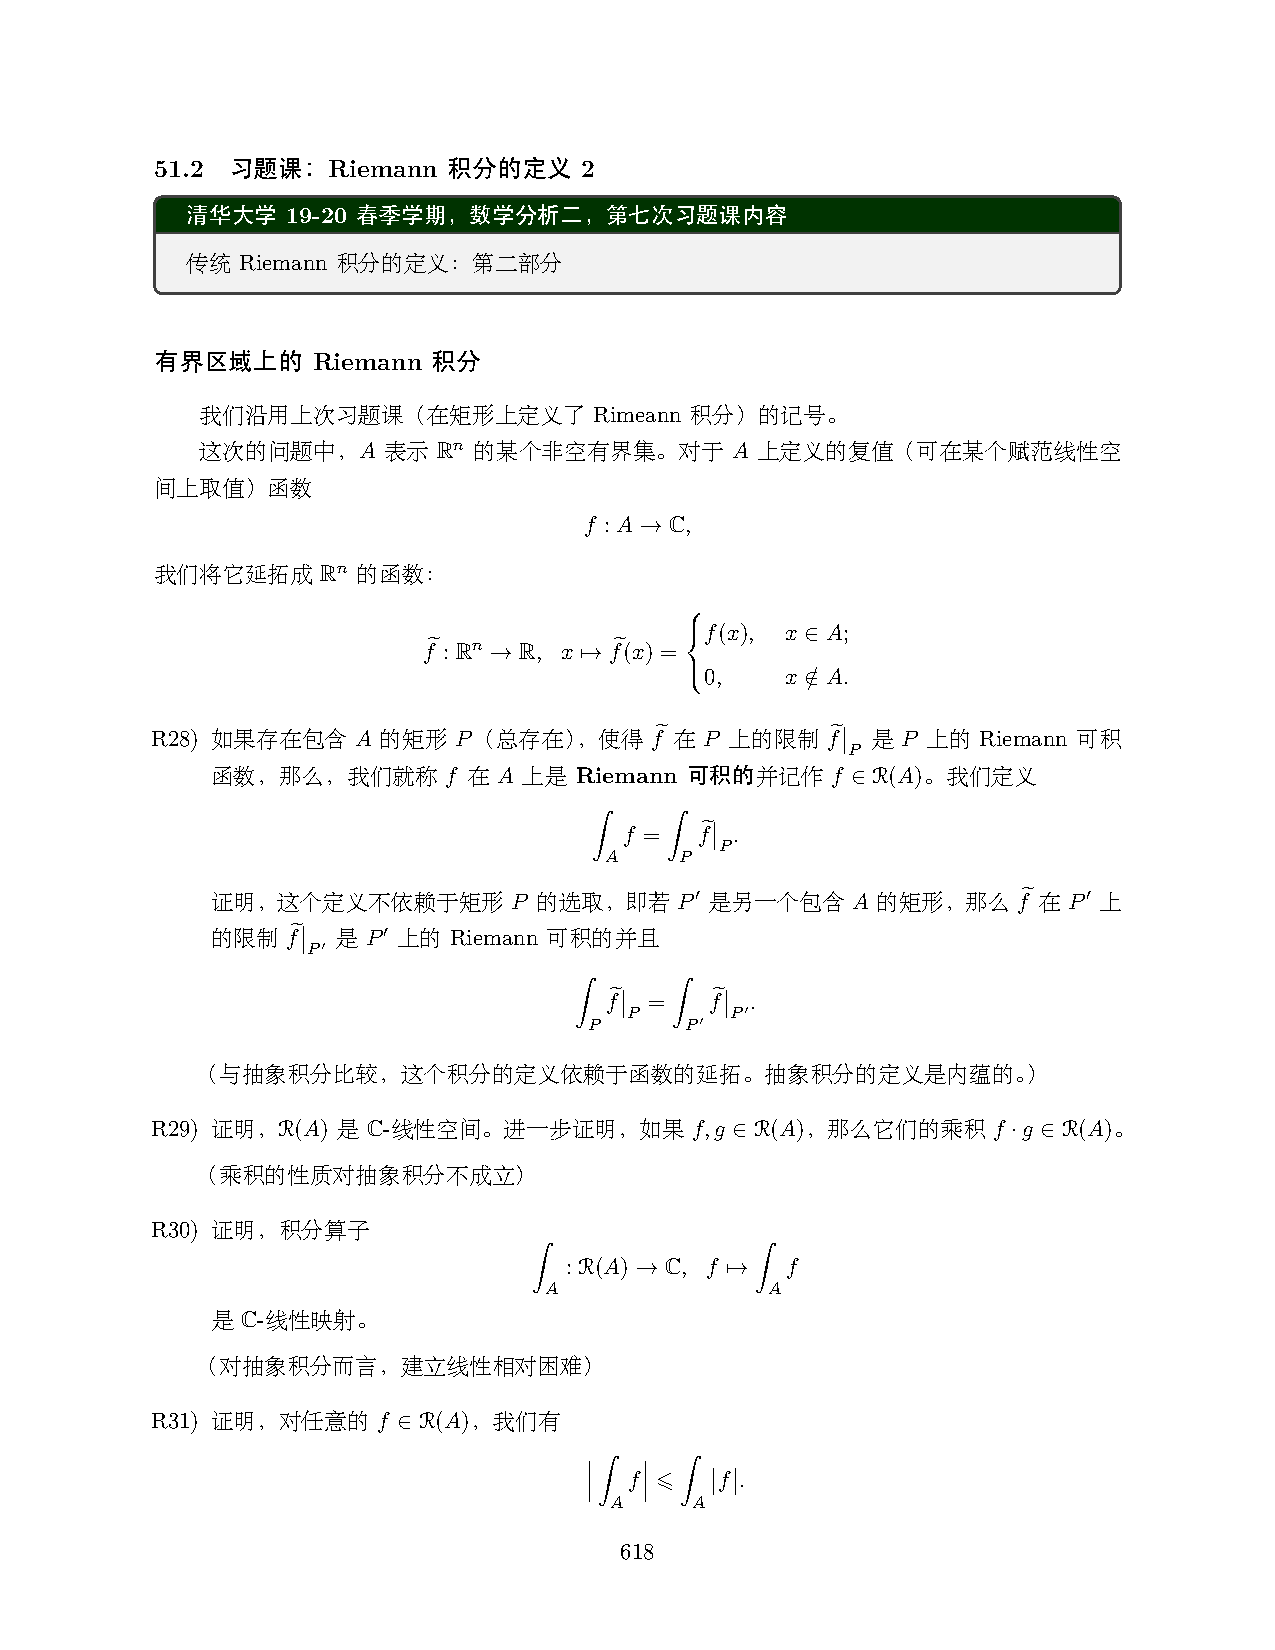
\includepdf[pages=-,pagecommand={\thispagestyle{empty}},scale=.94]{original.pdf}}

\begin{document}
\sourceintro{51.2 习题课：Riemann积分的定义2}{51.2}{618--622}
\section*{所用知识与记号}
沿用48.2的矩形积分理论。$A\subset\R^n$非空有界，$\widetilde f$表示$f$在$A$外延零。可铺集允许体积为零的退化矩形，见48.2 R3勘误。上、下积分记作$\overline I,\underline I$。抽象可铺即Jordan可测，不预先假定$A$为Borel集。原文没有R44，编号照录而不补造题目。
\section{有界集上的积分}
\problem{R28}{若某个矩形$P\supset A$上$\widetilde f$可积，定义$\int_Af=\int_P\widetilde f$。证明与$P$无关，且任意另一$P'\supset A$上也可积并取相同积分。}
取大矩形$Q\supset P\cup P'$，沿$P,P'$的边界作网格。将$\widetilde f|_P$延零到$Q$，边界外为零，由48.2 R16可积且积分不变。再限制到$P'$，其补格函数为零，R16又使积分等于$Q$上的值。相交面的赋值不影响积分。
\problem{R29}{证明$R(A)$为复线性空间且对乘积封闭。}
在共同大矩形上，延零与线性组合、乘积相容，直接用48.2 R12。
\problem{R30}{证明$\int_A:R(A)\to\C$线性。}
延零线性，矩形积分线性，由R28定义得到。
\problem{R31}{证明$|\int_Af|\le\int_A|f|$；实函数$f\le g$时积分保序。}
延零保持绝对值和次序，在共同大矩形上使用48.2 R15。
\problem{R32}{证明实可积$f,g$的最大值、最小值仍可积，且
\begin{align*}\int_A\min(f,g)&\le\min(\int_Af,\int_Ag),\\\max(\int_Af,\int_Ag)&\le\int_A\max(f,g).\end{align*}}
延零与最大最小相容；或者用$\max=(f+g+|f-g|)/2$和$\min=(f+g-|f-g|)/2$，再由逐点界及R31。
\problem{R33}{证明$|\int_Afg|\le(\int_A|f|^2)^{1/2}(\int_A|g|^2)^{1/2}$。}
把$f,g$延零至同一矩形，直接应用48.2 R27。
\problem{R34}{若$A$可铺，$f$实值Riemann可积，$c=\inf_Af,C=\sup_Af$，证明存在$\xi\in[c,C]$使$\int_Af=\xi m(A)$。}
由$c\ind_A\le\widetilde f\le C\ind_A$得$cm(A)\le\int_Af\le Cm(A)$。若$m(A)>0$取$\xi=\int_Af/m(A)$；若$m(A)=0$则积分为零，任选$\xi\in[c,C]$。不要求$\xi$为某个点的函数值。
\problem{R35}{若$f_k\in R(A)$一致收敛到$f$，证明$f\in R(A)$且$\int_Af=\lim_k\int_Af_k$。}
延零后在$P$上一致收敛。给定$\eps$先取$k$使$\norm{\widetilde f-\widetilde f_k}_\infty<\eps/(2m(P))$，再用$\widetilde f_k$的阶梯逼近，使误差积分小于$\eps/2$，相加得到$f$的可积性。且$|\int_A(f-f_k)|\le m(P)\norm{f-f_k}_\infty\to0$。若$m(P)>0$总可选择，故分母无问题。
\problem{R36}{对有界实$f:A\to\R$，用包含$A$的矩形$P$上超过或低于$\widetilde f$的阶梯函数定义上下积分。证明与$P$无关。}
在共同大矩形内比较。任一阶梯上界可限制到子矩形；反向可将子矩形上的上界延零，在其边界上取不小于$\widetilde f$的值。新增区域函数为零，积分不变。若边界网格不相容，先沿矩形端点共同加细；边界值体积为零。上下界的确界因此保持不变。
\problem{R37}{证明有界实$f$在$A$上可积当且仅当上下积分相等，此时共同值等于$\int_Af$。}
在任意固定$P\supset A$上应用48.2 R21--R22与R28、R36。
\section{抽象可铺集}
若$\ind_A\in R(P)$，称$A$抽象可铺，$m(A)=\int_P\ind_A$。
\problem{R38}{证明可铺集抽象可铺。}
示性函数在共同端点网格的每个开格上为常数，所以是阶梯函数。退化面的示性函数也为阶梯函数且积分零；由有限和或有限并得到结论。
\problem{R39}{若$A,B$抽象可铺，证明$A\cap B,A\cup B,A\setminus B$均如此，并证明体积的加法与差公式。}
用$\ind_{A\cap B}=\ind_A\ind_B$、$\ind_{A\cup B}=\ind_A+\ind_B-\ind_A\ind_B$、$\ind_{A\setminus B}=\ind_A-\ind_A\ind_B$，再用R29、R30。
\problem{R40}{对任意有界$A$，以上下积分定义上、下体积$\overline m(A),\underline m(A)$。证明$\overline m(A)=\inf_{B\supset A,\ B\text{可铺}}m(B)$，$\underline m(A)=\sup_{C\subset A,\ C\text{可铺}}m(C)$。}
第一项：任何有限矩形覆盖的并$B$给出阶梯上界$\ind_B$，故上积分不超过$m(B)$。反向对$\ind_A$取Darboux上和接近上积分的网格；把与$A$相交的所有闭格收集起来即得可铺覆盖，体积等于上和（格面零体积），所以取下确界一致。第二项：$C\subset A$时$\ind_C\le\ind_A$给出一向；反向，对近似下积分的网格，把完全位于$A$的闭格收集，得到体积等于相应Darboux下和的可铺子集。于是取上确界相同。此处上、下和以\emph{闭格}上的上、下确界定义，避免开格边界引起的误判。
\problem{R41}{原文要求证明：$A$抽象可铺当且仅当每个$\eps>0$存在可铺$B\supset A\supset C$使$m(C)-m(B)<\eps$。}
\fix{差的顺序反了，应为$m(B)-m(C)<\eps$。原式对任意有界$A$取大矩形$B$和$C=\varnothing$都成立，无法刻画可积性。}
R40给出$\underline m(A)\le\overline m(A)$。两者相等时分别选接近确界的$B,C$，使差$<\eps$；反向由差界夹住上、下体积，再令$\eps\to0$，用R37。
\problem{R42}{证明$A^\circ$是$A$内最大开集，$\overline A$是包含$A$的最小闭集；原文还称$\overline A$恰为聚点集。}
内部是所有包含在$A$中的开球之并，故开且最大。闭包的补集由与$A$不相交的开球组成，故开；任何含$A$的闭集也必须包含所有与$A$任意近的点，故最小。
\fix{若“聚点”采用标准的去心邻域定义，末句应为$\overline A=A\cup A'$。例如$A=\{0\}$的闭包是自身而聚点集为空。若作者把“聚点”用作附着点，则只是术语差异。}
\problem{R43}{令$\partial A=\overline A\setminus A^\circ$。证明$\ind_A$在$\R^n\setminus\partial A$连续。}
这些点或在$A^\circ$，邻域上恒为$1$；或在$\R^n\setminus\overline A$，邻域上恒为$0$。
\problem{R45}{证明有界$A$抽象可铺当且仅当$\partial A$为Lebesgue零测集。}
可由53.2 R53的Lebesgue判据立即得到，但这里给出直接几何证明。取包含$\overline A$于内部的矩形$P$。若$\partial A$零测，它是紧集，可用有限个开矩形覆盖且总体积任意小。细网格中所有同时击中$A$和其补集的闭格必击中边界，并在足够细时全落在该开覆盖内；其总体积任意小，故$\ind_A$的Darboux上下和差趋零。反向，选使上下和差$<\eps$的网格。边界点若不在网格面上，所在格必同时含$A$和补集，故所有边界包含在振幅为$1$的闭格与有限个网格面中；后者可用任意小总体积薄条覆盖。于是边界外测度至多$\eps$。令$\eps\downarrow0$即得零测。
\problem{R46}{若每个$\eps>0$均可用有限个矩形覆盖$A$且总体积$<\eps$，称$A$为R-零测集。证明它有界、Lebesgue零测，子集仍R-零测，有限并仍R-零测。}
取$\eps=1$的有限覆盖给出有界性。有限覆盖也是可数覆盖，故Lebesgue零测；子集继承覆盖；对有限并把误差配为$\eps/N$再合并覆盖。
\problem{R47}{证明R-零测集的闭包仍R-零测；证明$\Q\cap[0,1]$为Lebesgue零测但不R-零测。}
矩形取闭矩形，有限并闭，故覆盖$A$也覆盖$\overline A$，体积和不变。若有理点集R-零测，其闭包$[0,1]$也R-零测，与区间体积$1$和有限覆盖的体积次可加性矛盾。有理点集可数，故Lebesgue零测。
\problem{R48}{证明$\R^n$中紧的$d$维光滑子流形（$d<n$）为R-零测集。}
41.1 C4证明它是Lebesgue零测；取总体积$<\eps$的可数矩形覆盖，将每个矩形稍扩大成开矩形而使总体积仍$<\eps$，紧性给出有限子覆盖，故R-零测。
\problem{R49}{证明等价：(甲)$A$为R-零测；(乙)$A$抽象可铺且$m(A)=0$；(丙)$A$抽象可铺且Lebesgue零测；(丁)$A$有界且$\overline A$为Lebesgue零测。}
甲$\Rightarrow$乙：上体积由有限覆盖任意小而为零，下体积非负，所以可积且体积零。乙$\Rightarrow$丙：R40给出任意小的有限可铺覆盖，故Lebesgue零测。丙$\Rightarrow$丁：由R45，$\partial A$零测；又$\overline A\subset A\cup\partial A$，故闭包零测。有界性为抽象可铺定义的一部分。丁$\Rightarrow$甲：闭包紧且零测，如R48的开覆盖紧性论证，得到有限小体积覆盖。特别注意丁说的是\emph{闭包}零测，原文此处有上横线。
\problem{R50}{证明有界$A$抽象可铺当且仅当$\partial A$为R-零测。}
边界紧。由R45和紧零测集有限覆盖性质，Lebesgue零测与R-零测在边界上等价。
\originalpages
\end{document}
